% LuaLaTeXでの利用を想定
\documentclass[lualatex]{jlreq}

% 画像を利用するためのパッケージの読み込み
\usepackage{graphicx}
% figure環境を利用しつつ,その場に強制的に画像を表示したい場合
\usepackage{float}

\begin{document}
	% texファイルと同じディレクトリにsample.pngがある場合
	画像を貼りたい場合には
	\includegraphics{sample1.png}
	とします.

	% 別のディレクトリに画像がある場合
	% 画像を中央ぞろえにしてみる
	別のディレクトリに画像を配置した場合には
	\begin{center}
		\includegraphics{./picture/sample1.png}
	\end{center}
	とします.

	% 画像の大きさを指定する場合
	% 絶対値で高さを50mmにする場合
	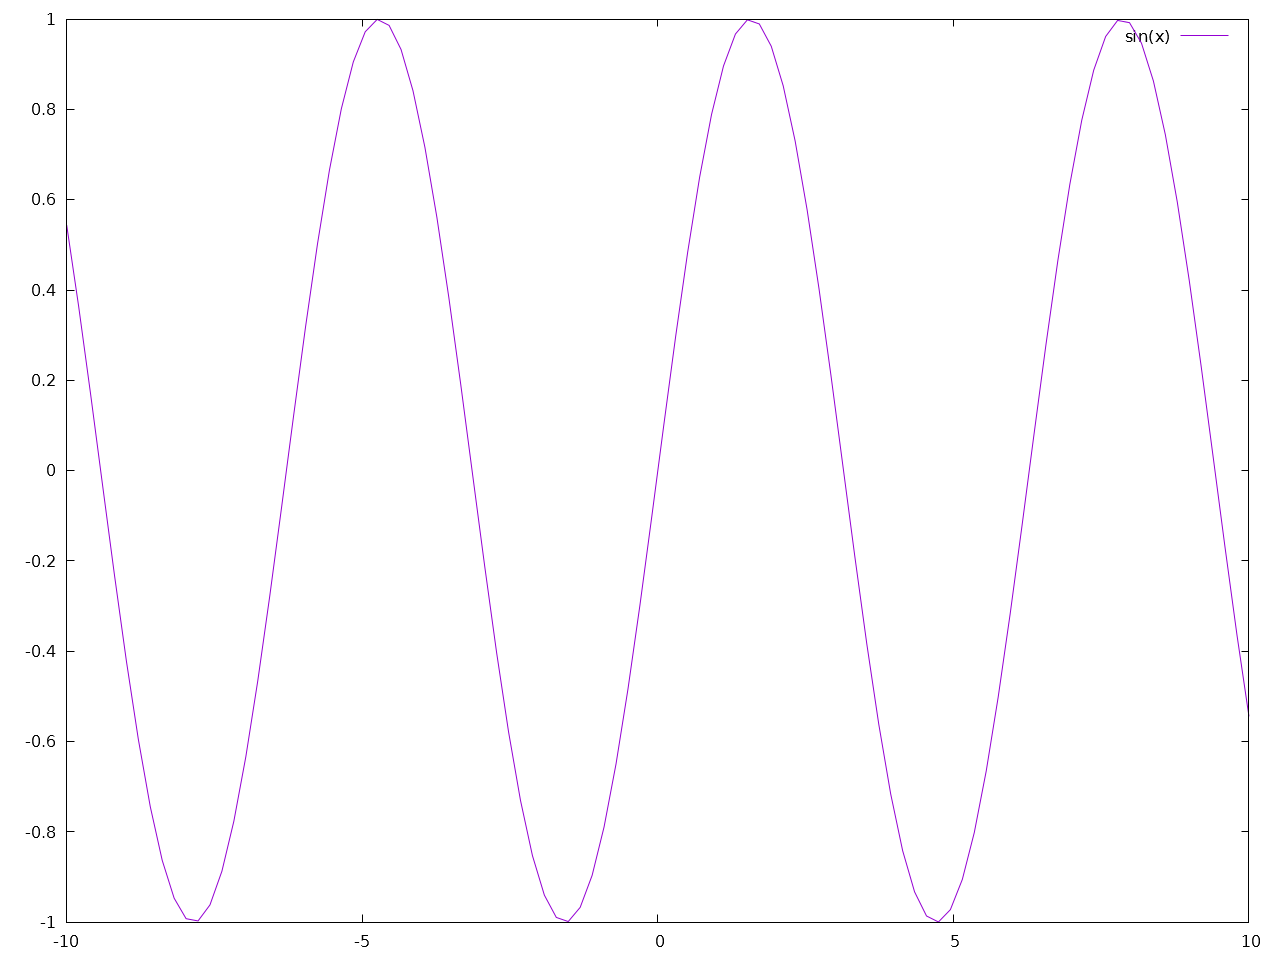
\includegraphics[height=50mm]{sample2.png}\\
	% 相対値で横幅を版面サイズの横幅の70%にする場合
	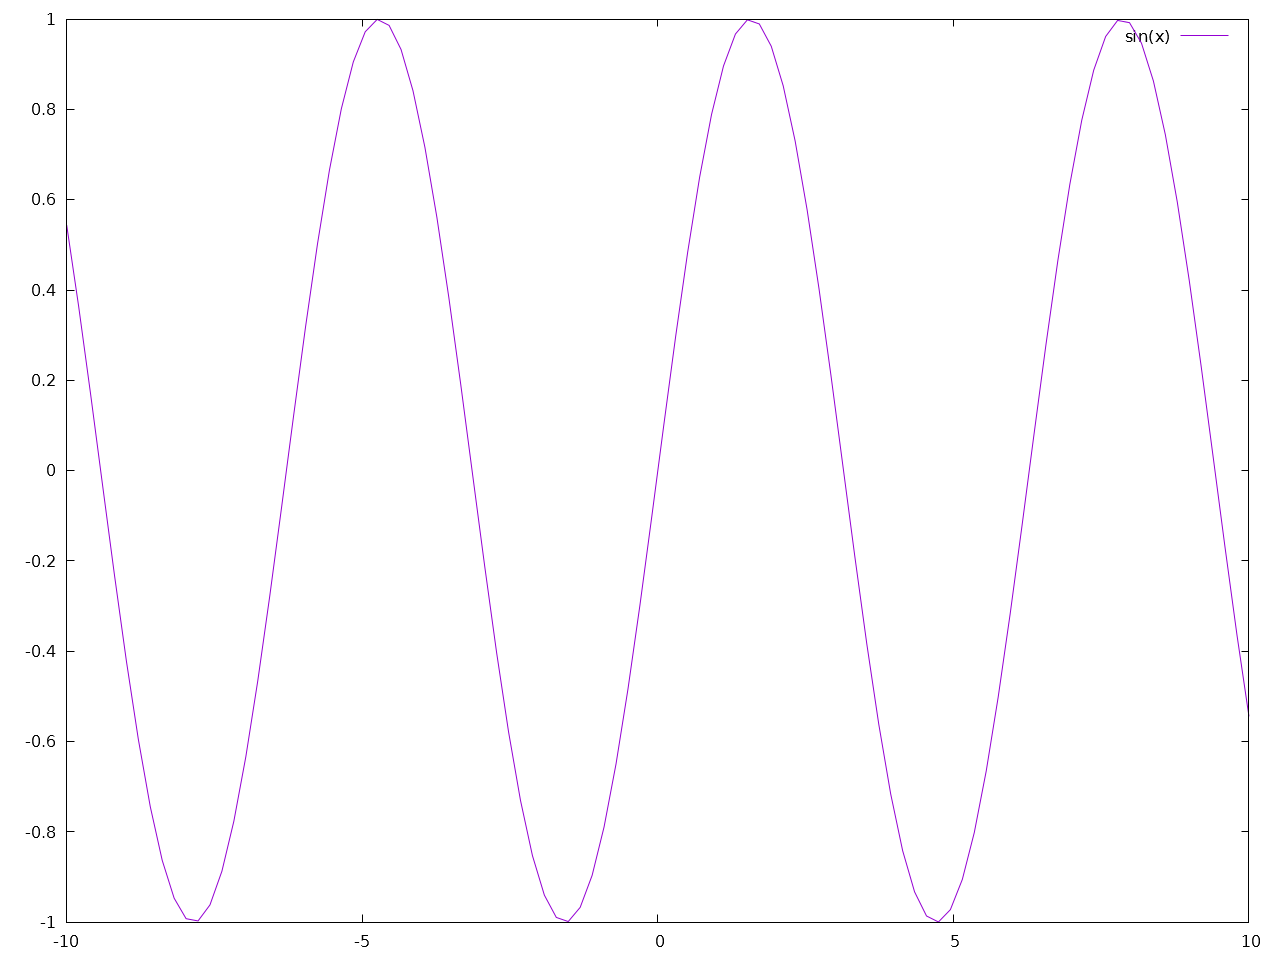
\includegraphics[width=0.7\columnwidth]{sample2.png}

	% 図の自動配置
	図\ref{fig:sample}はキャプションや参照の参考である.
	\begin{figure}[htbp]
		% 画像が中央に揃うようにする
		\centering
		% 画像を読み込む
		\includegraphics[width=.7\columnwidth]{sample1.png}
		% キャプションをつける
		\caption{適当なキャプション}
		% 本文中で画像を参照するための準備
		\label{fig:sample}
	\end{figure}

	% 図を横並びする例
	% 横並びさせたい画像をひとつのfigure環境にいれる
	% 2枚横並びにする場合
	\begin{figure}[H]
		\centering
		\begin{minipage}{0.4\columnwidth} % ひとつのminipageの幅を版面サイズの0.4倍とする
			\centering
			% 画像の横幅をminipageの1.0倍にする
			\includegraphics[width=\columnwidth]{sample1.png}
			\caption{sample1}
			\label{fig:sample1}
		\end{minipage}
			\begin{minipage}{0.4\columnwidth} % ひとつのminipageの幅を版面サイズの0.4倍とする
			\centering
			% 画像の横幅をminipageの1.0倍にする
			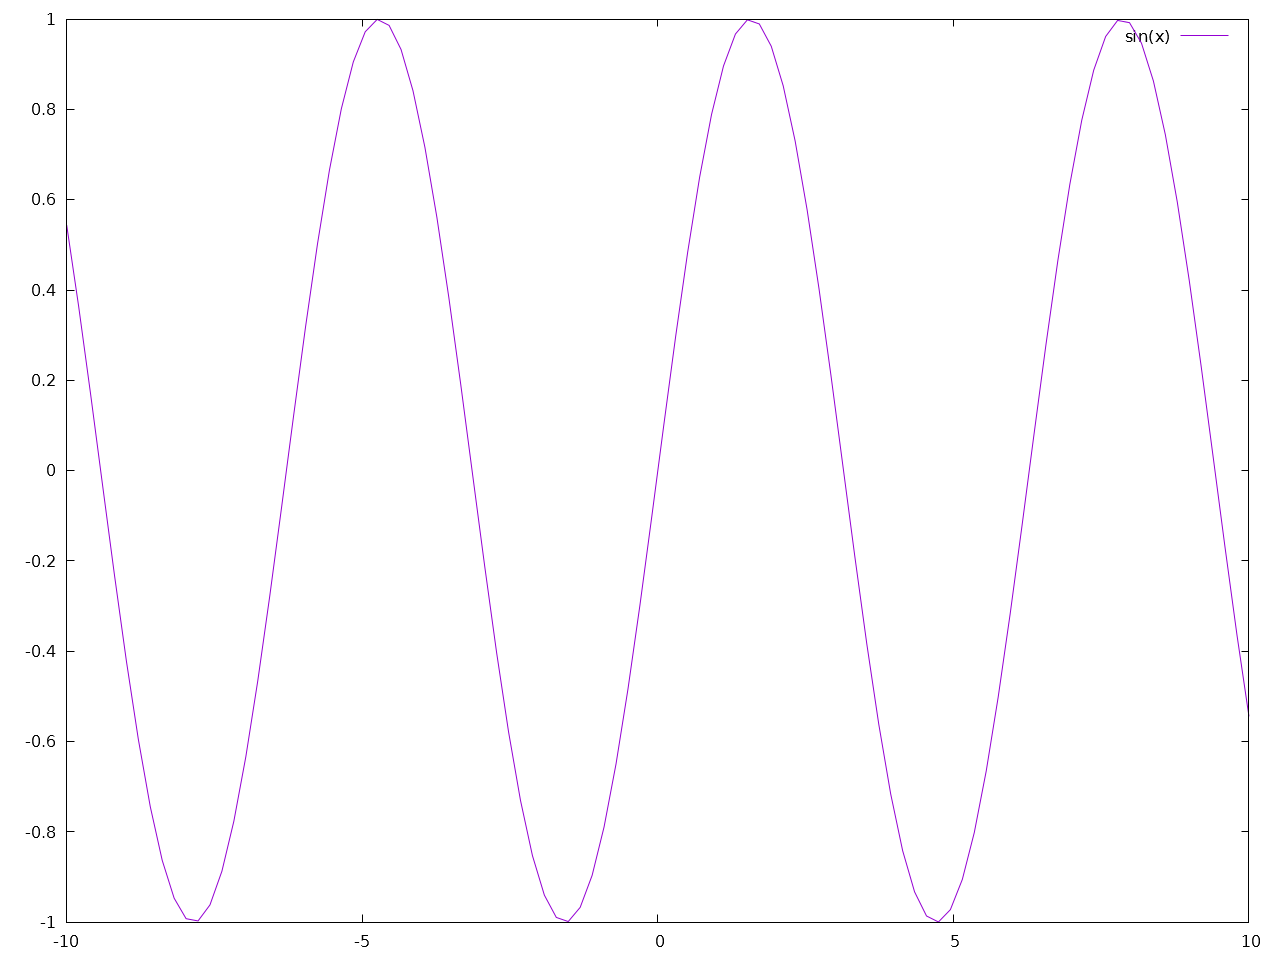
\includegraphics[width=\columnwidth]{sample2.png}
			\caption{sample2}
			\label{fig:sample2}
		\end{minipage}
	\end{figure}
\end{document}